\subsection{Stage 3: DFT Reference Calculations}
\label{sec:stage3}

The reference stage uses Quantum Espresso \citep{giannozzi2009} (version~7.5)
driven through the Atomic Simulation Environment \citep{ase2017}. Before any
production runs, the QE--ASE coupling was checked on bulk FCC aluminium with a
three-point test: the single-point SCF energy lands in the expected $-540$ to
$-530$\,eV window, the residual atomic forces stay below $0.01$\,eV/\AA, and
the stress tensor is diagonal. For each requested element the stage then
computes:

\begin{enumerate}
	\item the equilibrium lattice constant $a_0$, cohesive energy
	      $E_\mathrm{coh}$, and bulk modulus $B$ from a seven-point
	      equation-of-state scan fit to a Birch--Murnaghan curve
	      \citep{birch};
	\item an isolated-atom reference energy in a large empty box, used to turn
	      the bulk total energy into a true cohesive energy;
	\item the cubic elastic constants $C_{11}$ and $C_{12}$ from a
	      stress--strain calculation analogous to the LAMMPS protocol of
	      Section~\ref{sec:stage2}.
\end{enumerate}
For each unordered binary pair $(i,j)$ a single SCF run on the L1$_2$ or B2
reference structure (chosen from the lattice types of the two elements) gives
the formation energy $E_\mathrm{form}(i,j)$.

Plane-wave cut-offs are set per element, starting near $40$\,Ry and raised for
the harder pseudopotentials, with a charge-density cut-off of $320$\,Ry,
Marzari--Vanderbilt smearing \citep{marzari1999} of width $0.02$\,Ry, and a
$6\!\times\!6\!\times\!6$ Monkhorst--Pack mesh \citep{monkhorst1976}.
Pseudopotentials are pulled from the Quantum Espresso library on demand. The
EOS strain points and the binary SCF runs are dispatched to a process pool,
which made the full reference set tractable on a single workstation.

\paragraph{Magnetic elements.}
The 3$d$ transition metals Fe, Cr, and Mn need spin polarization, and a plain
collinear SCF for them tended to settle into the wrong magnetic state. These
elements were rerun with a fixed-moment SCF that constrains the total moment
during the self-consistency loop. Even so, the elastic-constant extraction for
Fe and Mn remains the weakest part of the reference set: the fitted
$(C_{11},C_{12})$ for both violate $C_{11}>C_{12}$ in
Table~\ref{tab:dft_elements}, so their cross-terms carry a higher uncertainty
into Stage~4 and are corrected there from $B$ and a Poisson-ratio default
(Section~\ref{sec:stage4}).

The current reference set covers ten elements (Al, Cu, Si, Ti, Zn, Cr, Fe, Mg,
Mn, Mo) and all $45$ of their binary pairs. The fitted elemental properties are listed in
Table~\ref{tab:dft_elements}, and the EOS fits are shown in
Figure~\ref{fig:eos}. The Mn row was kept at its tabulated value because the
EOS scan would not converge for the simplified $\alpha$-Mn approximation.

% AUTO-GENERATED by src/stats/ -- do not edit by hand
\begin{table}[h]
\centering
\caption{Elemental reference data extracted from DFT. $E_\mathrm{coh}$ is in eV/atom and $B,C_{ij}$ in GPa.}
\label{tab:dft_elements}
\begin{tabular}{llrrrll}
\hline
 Element   & Lattice   &   $a_0$ (\AA) &   $E_\mathrm{coh}$ &     $B$ & $C_{11}$   & $C_{12}$   \\
\hline
 Mg        & HCP       &         3.177 &              1.483 &  47.800 & 78.926     & 32.237     \\
 Mo        & BCC       &         3.169 &             10.353 & 280.800 & 407.600    & 63.200     \\
 Al        & FCC       &         4.047 &              3.611 &  77.500 & 167.100    & 32.600     \\
 Cu        & FCC       &         3.639 &              3.857 & 138.500 & 135.100    & 127.500    \\
 Zn        & HCP       &         2.766 &              0.964 &  68.400 & ---        & ---        \\
 Ti        & HCP       &         2.915 &              6.284 & 114.500 & ---        & ---        \\
 Si        & DIAMOND   &         5.471 &              5.130 &  89.300 & ---        & ---        \\
 Co        & HCP       &         2.488 &              5.630 & 222.600 & ---        & ---        \\
 Cr        & BCC       &         2.851 &              3.971 & 256.700 & ---        & ---        \\
 Fe        & BCC       &         2.837 &              4.928 & 221.600 & ---        & ---        \\
 Mn        & BCC       &         2.830 &              3.731 & 166.100 & ---        & ---        \\
 Ni        & FCC       &         3.521 &              4.729 & 200.300 & ---        & ---        \\
\hline
\end{tabular}
\end{table}


\begin{figure}[htbp]
	\centering
	
\includegraphics[width=0.85\textwidth]{figures/eos_curves.png}
	\caption{Birch--Murnaghan fits to the seven-point DFT equation-of-state
	scans. The fitted minimum sets $a_0$ and $E_\mathrm{coh}$; the curvature
	sets $B$.}
	\label{fig:eos}
\end{figure}

The 45 binary formation energies $E_\mathrm{form}(i,j)$ are summarized as a
symmetric heatmap in Figure~\ref{fig:formation}. Negative values (blue) mark
exothermic mixing, as expected for compatible pairs such as Al--Ti or Cu--Ti,
while strongly positive values (red) flag low mutual solubility, most visibly
for Mg and Zn against the transition metals. These signed values feed the
cross-term seeding of Stage~4 directly and propagate unchanged into the
$E_c(i,j)$ entries of the merged MEAM library.

\begin{figure}[htbp]
	\centering
	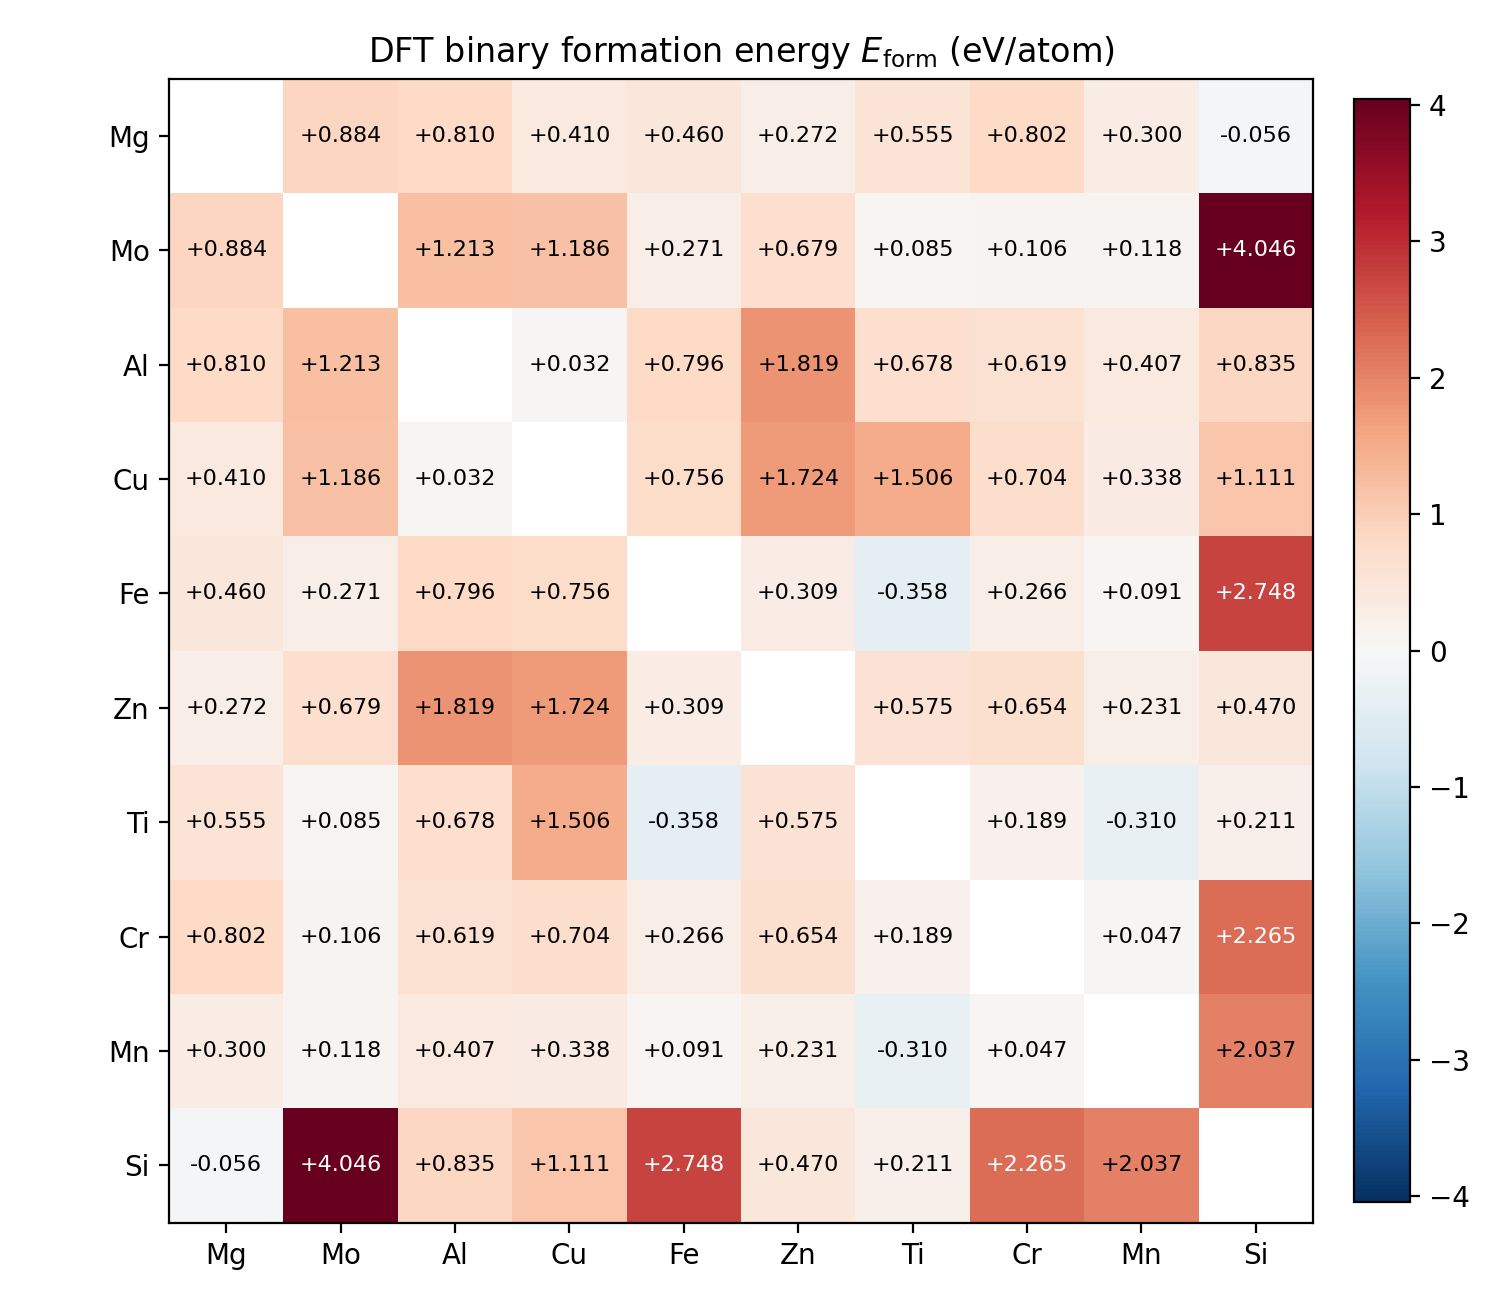
\includegraphics[width=0.92\textwidth]{figures/formation_energy_heatmap.png}
	\caption{DFT binary formation energy $E_\mathrm{form}(i,j)$ in eV/atom for
	the ten elements with a converged elemental reference. The matrix is
	symmetric by construction; the diagonal (self,self) entries are not
	computed and are left blank.}
	\label{fig:formation}
\end{figure}
